\setcounter{footnote}{0}
\renewcommand{\thefootnote}{[\roman{footnote}]}
\setlength{\footnotesep}{\baselineskip}
\tfarsi{%
\te{\raisebox{1.75ex}{\color{darkgray}$\neg$}}\kern-.75ex\tfarsib{باب ششم}\te{\marginnote{\te{\raisebox{1.75ex}{\color{darkgray}$\neg$}}\footnotesize f.~21b:\thinspace 20~\SjA\ \&\\
\hspace{8pt}f.~16a:\thinspace 25~\SjB}}\\
در معرفت بعد كواكب از معدّل النهار.\hfill}
\bigskip


\tfarsi{%
عرض کوکب و میل ثاني درجه او، %
اگر هر دو در یک جهت باشند
جمع کنیم والا تفاضل بگیریم  و آن را حصّه بعد خوانیم  و جهت حصّه بعد
جهت مجموع یا جهت فضل باشد.\te{(1)}\hfill}


\tfarsi{%
پس جيب حصّه بعد را در جیب تمام
میل منکوس درجه كوكب منحطّ ضرب کنیم حاصل جيب % 
\te{\raisebox{1.75ex}{\color{darkgray}$\neg$}}\kern-.75ex
بعد %
\te{\marginnote{\te{\raisebox{1.75ex}{\color{darkgray}$\neg$}}\footnotesize f.~22a:\thinspace 1~\SjA}}%
بود.\te{(2)}\hfill}
\bigskip

\tfarsi{%
بوجهی\te{\footnote{ %
\tfarsi{بوجهی}  {\normalsize ]}  \raisebox{-.6ex}{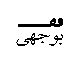
\includegraphics[scale=.85]{Images/qif_over_text_logograph.eps}}~\SjA. The overlining `
\includegraphics[scale=0.85]{Images/qif_arabic_logograph.eps}' over the word \tfarsi{بوجهی} is used to indicate a notable pause in the reading. As \textcite[173]{Gacek} explains, it is most likely a logograph (word-symbol) of the Arabic word \tfarsi{قف} (\qif) `stop' to indicate a pause in reading; or alternatively, the abbreviation \tfarsi{فتــ‬} (\textit{fata--}) of the phrase \tfarsi{فتأملها} (\fatammalha)
`reflect on it'.\label{qif_overlinning}}}
دیگر جيب حصّه بعد را در جیب تمام میل کلّی ضرب کنیم
و حاصل را بر جيب تمام میل\te{\footnote{ % 
\tfarsi{میل} {\normalsize ]} \tfarsi{%
میل \cancel{کلّی}}~\SjA, cancellation \textit{intra lineam}.}}
ثاني درجه آن کوکب قسمت کنیم
خارج  
\te{\raisebox{1.75ex}{\color{darkgray}$\neg$}}\kern-.75ex
قسمت %  
\te{\marginnote{\te{\raisebox{1.75ex}{\color{darkgray}$\neg$}}\footnotesize f.~16b:\thinspace 1~\SjB}}%
جيب بعد باشد و جهت آن جهت حصّه بعد باشد.\te{(3)}\hfill}


\tfarsi{%
و چون جيب حصّه بعد را در جدول جيب تمام میل کلّی درآرند و حاصل را بر جيب تمام میل ثاني درجه آن کوکب  قسمت کنند خارج قسمت جيب بعد باشد.\te{(4)}\hfill}

\tfarsi{%
و اگر کوکب را عرض نباشد، میل درجه او بعد باشد.\te{(5)}\hfill}

\tfarsi{%
و اگر عرض باشد اما درجه او را میل نباشد، جيب عرض او را در جیب تمام میل كلّی منحطّ ضرب کنیم
یا در\te{\footnote{ %
\tfarsi{یا در} {\normalsize ]} 
\tfarsi{یاد در}~\SjB, dittography of the first \tfarsi{د}.}}   
جدول سابق درآریم
حاصل جيب بعد باشد و جهت او جهت عرض باشد.\te{(6)}\hfill}

\tfarsi{%
و اگر میل درجه او میل كلّی باشد، حصّة البعد بعينه بعد باشد.\te{(7)}\hfill}
\newpage

\tfarsi{%
و بوجهی\te{\footnote{ %
\tfarsi{و بوجهی} {\normalsize ]} 
\raisebox{-.6ex}{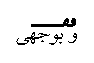
\includegraphics[scale=.85]{Images/qif_over_text_logograph_2.eps}}~\SjA, with emphasis. \Vid\ footnote~\ref{qif_overlinning}.}}
دیگر جيب بعد درجه کوکب از انقلاب اقرب در جیب
تمام عرض کوکب منحطّ ضرب کنیم حاصل جیب بعد کوکب از
دایرهٔ ماره باقطاب اربعه %
\wrapfootnote{%
باشد.\nobreak\te{(8)}\hfill\break
\te{\phantom{a}}\break % Required to allow a line break within a single \tfarsi{} group (Hack!)
پس جیب عرض کوکب را بر جيب تمام بعد از دایرهٔ ماره باقطاب اربعه}%
{ %
\tfarsi{باقطاب اربعه}%
\thinspace\dots\thinspace
\tfarsi{باشد.\@  پس} 
\te{\normalsize ]}
\begin{itemize}
    \item 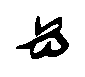
\includegraphics[height=.75em]{Images/marginal_insertion_end.eps}~~%
\tfarsi{باقطاب اربعه}%
\thinspace\dots\thinspace
\tfarsi{پس} %
$\stackrel{\text{\tiny\signederenvoi}}{\text{\tfarsi{باشد}}}$~\SjA, %
inserted in the exterior margin by the same hand.
The penultimate word of passage~(8) on f.~22a:\thinspace 6  has 
an insertion mark `\signederenvoi' (\textit{signe-de-renvoi}) placed above it, \scl  \dots\thinspace\tfarsi{منحطّ} %
$\stackrel{\text{\tiny\signederenvoi}}{\text{\tfarsi{اربعه} }}$ %
\tfarsi{باقطاب}\thinspace\dots\thinspace .  
The first word of the marginal text also bears the same mark, \textit{supra verbum}, \scl\ \dots\thinspace
\tfarsi{پس} %
$\stackrel{\text{\tiny\signederenvoi}}{\text{\tfarsi{باشد}}}$. The marginal text ends with  `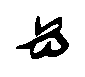
\includegraphics[height=.75em]{Images/marginal_insertion_end.eps}': this could be a calligraphic variant of the abbreviation \tfarsi{هى} (\textit{hā}\Ayn) of the Arabic word \tfarsi{إنتهى} (\intiha) meaning `it is finished', \vid\ \textcite[117]{Gacek};
\item \tfarsi{باقطاب اربعه}%
\thinspace\dots\thinspace
\tfarsi{باشد.\@  پس}~\textit{omitted} \SjB,  per homeoteleuton. The penultimate word \tfarsi{\underline{اربعه}} of passage~(8), %
before the missing text, is identical to the last word of the missing text %
\tfarsi{\underline{اربعه} منحطّ\thinspace\dots}\thinspace %
 in  passage~(9). \textbf{\scshape remark}: MS~UbC of the \ZijUlughBeg\ is also missing the same text, \viz \tfarsi{باشد\thinspace\dots\thinspace اربعه} %
spanning the length of a line between the end of line 18 (at \tfarsi{اربعه}) %
and the beginning of line 19 (at \tfarsi{منحطّ}) on folio 16r.
\end{itemize}\vspace{-\topsep}
} %
منحطّ قسمت کنیم %
\wrapfootnote{و به خارج قسمت}%
{\tfarsi{%
و~به~خارج~قسمت
}\te{\normalsize ]} \tfarsi{
و به خارج قسمت کنیم  و به خارج قسمت
}~\SjB, dittography of the second \tfarsi{و به خارج قسمت}. %
I suspect a parableptic error as the word \tfarsi{قسمت} %
appears twice on the line in close proximity: 
\dots\thinspace \tfarsi{\underline{قسمت} از}\thinspace\dots\thinspace\tfarsi{\underline{قسمت} کنیم}\thinspace\dots\thinspace.}
از جدول جيب قوس بگیریم و آن را قوس اوّل خوانیم  و جهت آن جهت عرض کوکب بود.\te{(9)}\hfill}


\tfarsi{%
پس اگر عرض و میل درجه كوكب هر دو در یک جهت باشند، قوس اوّل و میل كلّی را جمع کنیم. و اگر از 
ربع\te{\footnote{ %
\tfarsi{ربع} {\normalsize ]}  
\begin{itemize}
    \item \tfarsi{بع}\cancel{\tfarsi{ا}}\tfarsi{ر}~\SjA,  erasure
\textit{intra lineam};
    \item \tfarsi{رابع}~\SjB. The Arabic words \tfarsi{ربع} (\rub) and \tfarsi{رابع} (\rabi) are the fractional (`one-fourth') and ordinal (`fourth') forms of the number four \tfarsi{أربعة} (\arbai) respectively. The mathematical context of the passage supports the fractional meaning `one-fourth' or a `quarter'. The reading in \SjB\ could be a semantic mistake by the scribe in copying Arabic loanwords (\moarrab).
\end{itemize}\vspace{-\topsep}}}
دور زیاده شود، تمام مجموع تا نصف دور بگیریم. و اگر در جهت مختلف باشند، تفاضل میان هر دو بگیریم حاصل قوس دوم باشد و جهتش جهت مجموع یا جهت فضل باشد.\te{(10)}\hfill}

\tfarsi{%
پس جیب قوس دوم را در جیب تمام بعد از
دایرهٔ ماره باقطاب اربعه منحطّ ضرب کنیم حاصل جيب بعد کوکب باشد  و جهتش جهت قوس دوم باشد.\te{(11)}\hfill}
